\documentclass[11pt, oneside]{article}   	% use "amsart" instead of "article" for AMSLaTeX format


%\usepackage{draftwatermark}
% \SetWatermarkText{Confidential}
% \SetWatermarkScale{5}
% \SetWatermarkLightness {0.85} 
% \SetWatermarkColor[rgb]{0.7,0,0}


\usepackage{geometry}                		% See geometry.pdf to learn the layout options. There are lots.
\geometry{letterpaper}                   		% ... or a4paper or a5paper or ... 
%\geometry{landscape}                		% Activate for for rotated page geometry
%\usepackage[parfill]{parskip}    		% Activate to begin paragraphs with an empty line rather than an indent
\usepackage{graphicx}				% Use pdf, png, jpg, or eps� with pdflatex; use eps in DVI mode
								% TeX will automatically convert eps --> pdf in pdflatex		
\usepackage{amssymb}
\usepackage{hyperref}
\usepackage{url}
\usepackage{authblk}
\usepackage{amsmath}
\usepackage{graphicx}
\usepackage{fixltx2e}
\usepackage{hyperref}
\usepackage{alltt}
\usepackage{color}


\title{Can Congestion in Data Center Networks Be\\Predicted By Of Time Of Day?\\\normalsize{Draft 0.0}}

\author{David Meyer \\ dmm@brocade.com}

% \date{}							% Activate to display a given date or no date


\begin{document}
\maketitle
\begin{abstract}

The recent explosive growth in data center structure, function and scale has brought a myriad of new challenges to network operators, including virtualization, development of new services, and the general scaling of data center capacity. These challenges share a common implication: network congestion (and hence network delay) within a data center has is strongly negatively correlated with  user quality of experience and operator efficiency. Hence congestion and the closely related problem of network delay are among the key concerns for data center and service operators.  Much of the literature in this area generally puts a finer point on the problem: a user's quality of experience can be badly affected when even a single flow suffers from a large latency~\cite{WILSON2011}. The work described in this document demonstrates a novel approach to the congestion control problem, namely, the use of artificial neural networks to predict nascent congestion (and hence queuing delay) in data center networks. This capability  will allow operators to both operational and capital expenditures while at the same time optimizing users' quality of experience. Our longer term goal is to build general framework for predicting various data center network parameters that effect both operator efficiency and user quality of experience.

\end{abstract}
\section{Introduction} 
\label{sec:intro}
%\subsection{}

The recent explosive growth in data center structure, function and scale has brought a myriad of new challenges to network operators, including virtualization, development of new services, and the general scaling of data center capacity. These challenges share a common implication: network congestion (and hence network delay) within a data center has is strongly negatively correlated with  user quality of experience and operator efficiency. Hence congestion and the closely related problem of network delay are among the key concerns for data center and service operators.  Much of the literature in this area generally puts a finer point on the problem: a user's quality of experience can be badly affected when even a single flow suffers from a large latency~\cite{WILSON2011}. 

The largest part of network delay in today's data centers comes from the queueing delay at router and switch interfaces. Since the propagation delay within a data center is in most cases negligible (in the ideal case a 100 meters of network cabling between two nodes adds only 0.5 $\mu$s of propagation delay, while a single 1500 byte packet queued at a 10Gbps port already costs 1.2 $\mu$s), managing delay is largely about reducing congestion and hence queuing delay at switch interfaces. For example, DCTCP~\cite{DCTCP} uses ECN marking to slow down flows before the relevant queues become full, while HULL~\cite{HULL} takes a further step and gives up a small amount bandwidth for even lower latency. Our work is also motivated by the need to reduce the queueing delay in data centers, but here we focus on predicting nascent congestion on important data center links as a method to minimize queuing delay. In this work we demonstrate a novel use of Artificial Neural Networks to predict nascent congestion (and hence queuing delay) in data center networks, which will allow operators to further optimize both operational and capital expenditures. Our longer term goal is to build general framework for predicting various data center network parameters that effect both operator efficiency and user quality of experience.

\subsection{Why Artificial Neural Networks?}

Recent advances in machine learning, coupled with the onslaught of data being collected from a wide variety of sensors has rekindled interest in using machine learning as a method to uncover hidden structure in these ever growing data sets\footnote{This  phenomena is evidenced by the explosive growth in the number of "data analytics" startups~\cite{ANALYTICS}.}. In particular, advances in the design of multi-layer deep artificial neural networks (DNNs) combined with effective approaches for training DNNs has opened up the opportunity to use DNNs for novel applications ranging from speech recognition and generation to self-driving vehicles. DNNs are  multiple-layer architectures (deep architectures) which extract inherent features in data and  discover important hidden structure in diverse data sets. Given that the factors contributing to traffic flow, congestion, and queuing delay in a data center result from the non-obvious interaction of complex factors, DNNs represent a novel and powerful method for learning how these factors interact and for predicting a wide variety of complex network behaviors. 

Neural networks had traditionally been trained with an algorithm called back propagation~\cite{WIDROW2002}, which is so named because the algorithm propagates the error in the neural network's estimate \emph{backward} from the output layer towards the input layer. Back propagation also requires labeled data sets; these \emph{training} sets have elements of the form $(\mathbf{x}^{(i)},\mathbf{t}^{(i)})$, where the $\mathbf{x}^{(i)}$ are the inputs and the $\mathbf{t}^{(i)}$ are the targets (the targets tell what the data is, for example, "cat"). The DNN computes an output value, sometimes called (largely for historical reasons) the hypothesis  $h_\theta(\mathbf{x}^{(i)})$.  $h_\theta(\mathbf{x}^{(i)})$  is then compared to the target $\mathbf{t}^{(i)}$ and the difference $h_\theta(\mathbf{x}^{(i)}) - \mathbf{t}^{(i)}$  is taken as an estimate of the model's error. This error is then "back propagated" (with the help of additional algorithmic machinery) down the DNN from output to input, adjusting the model parameters along the way. Back propagation is an instance of a  \emph{supervised learning} algorithm since it requires labeled data. Training algorithms that use unlabeled data are referred to as \emph{unsupervised learning} algorithms.

There were, however, several weaknesses with the back propagation algorithm which essentially limited the utility of DNNs. These included the fact that back propagation really didn't work well in deep networks (for technical reasons relating to the computation of what are called gradients) and the tendency for the algorithm to fall into poor local minima when the DNN was initialized with random weights\footnote{The problem of non-optimal minima is a property of non-convex optimization, where local minima aren't necessarily global minima when the some of the DNNs parameters were initialized with random values~\cite{CHIANG2011}.}. The requirement for labeled data sets was also a problem since most data is unlabeled.  These two problems with DNNs,  the need for labeled training sets and ineffective training via back propagation, were largely overcome by the groundbreaking work of Geoffrey Hinton and his colleagues in 2006~\cite{HINTON2006}. Hinton's breakthrough was to show that unsupervised, greedy, layerwise training of DNNs was effective in overcoming the problems with traditional back propagation training. This is discussed in more detail in Section~\ref{sec:sae}.

In this work we introduce the novel use of a specific form of DNN, the Stacked Autoencoder~\cite{VINCENT2008}, as a platform for predicting parameters of interest for data center and service operators, starting with congestion of important links in the data center. To demonstrate the technique, we attack the initial problem from the perspective of modeling congestion as a function of time of day; we call this problem the Spatial-Temporal Prediction of Traffic Flows in Data Centers Problem. The remainder of this paper is organized as follows: Section~\ref{sec:stptf} describes the Spatial-Temporal Prediction of Traffic Flows Problem in a data center network. Section~\ref{sec:methodology} describes our methodology and reviews both autoencoder and stacked autoencoder technology. Section~\ref{sec:datasets} outlines our data sets, evaluation metrics and results. Finally, Section~\ref{sec:conclusions} discusses conclusions and future work.

\section{The Spatio-Temporal Prediction of Traffic Flow Problem} 
\label{sec:stptf}
The Spatio-Temporal Prediction of Traffic Flow Problem is a formal description of the question asked in the title of this document and can be stated as follows: Let $X_{i}^{t}$ denote the the observed traffic flow during the $t^{th}$ time interval at the $i^{th}$ observation location. An observation location can be an interface counter, switch cpu load or memory utilization, or other relevant sensor value (note here that we consider traditional network interface counters to be \emph{sensors}). The network topology is not explicitly represented but is rather encoded in the observation locations. Now, given a sequence $\{X_{i}^{t}\}$ of observed traffic flow data , $i = 1, 2, ..., m$ and $t = 1, 2, ..., T$, the problem is to predict the traffic flow (and hence potential congestion) at the time $(t + \Delta)$ for some prediction horizon $\Delta$.  We also want to consider the temporal relationships inherent in traffic flows, so in order to predict the traffic flow at time interval $t$, we also use the traffic flow data at previous time intervals, i.e., $X^{t-1}, X^{t-2}, . . . , X^{t-r}$ for some value of $r$ (its not clear how far back in time you need to go to get valuable predictions). 

\section{Methodology} 
\label{sec:methodology}
In this section we introduce our basic methodology which is based on a deep-learning based prediction model. A stacked \emph{autoencoder}~\cite{BENGIO2007} model is used to learn generic traffic flow features. This section reviews basic autoencoder and stacked autoencoder technology. 

\subsection{The Basic Autoencoder}
\label{sec:basic}
The traditional autoencoder is an artificial neural network that attempts to reproduce its input, i.e., the target output is the input.  More formally (and following the notation of~\cite{VINCENT2008}), an autoencoder takes an input vector $\mathbf{x} \in [0,1]^d$ and maps it to a hidden representation $\mathbf{y} \in [0,1]^d$ through a deterministic mapping $\mathbf{y} = f_{\theta}(\mathbf{x}) = s(\mathbf{Wx} + b)$, parameterized by $\theta = \{\mathbf{W,b}\}$. $\mathbf{W}$ is a $d^\prime \times d$ weight matrix, $\mathbf{b}$ is a bias vector and $s$ is the \emph{sigmoid}\footnote{Note that the sigmoid activation function $s$ "squashes" its input into the range $[0,1]$} activation function, $s(\mathbf{x}) = \frac{1}{1 + e^{-\mathbf{x}}}$. The hidden representation $\mathbf{y}$, sometimes called the \emph{latent} representation,  is then mapped back to a �reconstructed� vector $\mathbf{z} \in [0,1]^d$, where  $\mathbf{z} = g_{\theta\prime}(\mathbf{y}) = s(\mathbf{W}^\prime\mathbf{y} + \mathbf{b}^\prime)$, with $\theta^\prime = \{\mathbf{W}^\prime, \mathbf{b}^\prime\}$. This scenario is depicted in cartoon form in Figure~\ref{fig:autoencoder}. Thus each training $\mathbf{x}^{(i)}$ is thus mapped to a corresponding $\mathbf{y}^{(i)}$ and a reconstruction (of $\mathbf{x}^{(i)}$) $\mathbf{z}^{(i)}$.  Finally, note that  the weight matrix $\mathbf{W}^\prime$ may optionally be constrained by $\mathbf{W}^\prime = \mathbf{W}^{T}$, in which case the autoencoder is said to have \emph{tied} weights. Each training example $\mathbf{x}^{(i)}$ is thus mapped to a corresponding $\mathbf{y}^{(i)}$ which is then mapped to a reconstruction $\mathbf{z}^{(i)}$ such that $\mathbf{z}^{(i)} \approx \mathbf{x}^{(i)}$.  

The basic idea here is that the autoencoder is constructed in such a way that the mapping $\mathbf{x}^{(i)} \mapsto \mathbf{y}^{(i)}$ reveals essential structure in the input vector $\mathbf{x}^{(i)}$ that is not otherwise obvious. For example, if the autoencoder has fewer hidden units than input units it must find a representation that essentially compresses the input in such a way that it can be efficiently reconstructed. The compressed representation has lower dimensionality than the input and is represents an \emph{abstraction} of the input. In the case of image recognition  $\mathbf{x}^{(i)}$ might be an image (pixels) while $\mathbf{y}^{(i)}$ might consist of edges in various orientations.

\begin{figure}[here]
\center{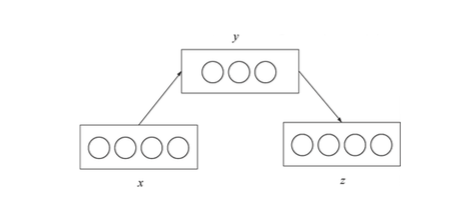
\includegraphics{autoencoder.png}}
\caption{Classic Autoencoder}
\label{fig:autoencoder}
\end{figure}


The parameters $\theta$ and $\theta^{\prime}$ of the model are optimized to minimize the \emph{average reconstruction error} as shown in Equation~\ref{eqn:loss}:

\begin{equation}
\begin{split}
\theta^{*}, \theta^{\prime *} = \operatorname*{arg\,min}_{\theta,\theta^\prime} \frac{1}{n}\sum\limits_{i = 1}^{n}L\left(\bold{x}^{(i)},\bold{z}^{(i)}\right) \\
 = \operatorname*{arg\,min}_{\theta, \theta^{\prime}} \frac{1}{n}\sum\limits_{i = 1}^{n}L\left(\mathbf{x}^{(i)}, g_{\theta^\prime}(f_\theta(\mathbf{x}^{(i)})\right)
\end{split}
\label{eqn:loss}
\end{equation}


Here $L$ is a loss function such as the traditional squared error $L(\mathbf{x}, \mathbf{z}) =   \parallel \mathbf{x} -  \mathbf{z}\parallel^{2}_{2}$. Note that if  $\mathbf{x}$ and $\mathbf{z}$ can be interpreted as either bit vectors or vectors or probabilities (i.e., they are Bernoulli probability vectors), then the \emph{reconstruction cross-entropy}, as defined in Equation~\ref{eqn:cross-entropy}, can be used.

\begin{equation}
\begin{split}
L_{\mathcal{H}}(\mathbf{x},\mathbf{z}) = \mathcal{H}(\mathcal{B}_\mathbf{x},\mathcal{B}_\mathbf{z}) \\
= - \sum\limits_{k = 1}^{d}[\mathbf{x}_k \log \mathbf{z}_k + (1 - \mathbf{x}_k) \log (1 - \mathbf{z}_k)]
\end{split}
\label{eqn:cross-entropy}
\end{equation}

More generally, this methodology casts learning as \emph{optimization} using Empirical Risk Minimization~\cite{BENGIO2013}. The Empirical Risk $\hat{R}$ is defined as
\begin{equation}
\hat{R}(f_\theta,D_n) = \sum\limits_{i = 1}^{n}L\left(f_\theta(\mathbf{x}^{(i)}), \mathbf{z}^{(i)}\right)
\label{en:empirical-risk}
\end{equation}
In some cases  It may be necessary to induce a preference for some values of the parameters to avoid �overfitting�~\cite{DIETTERICH95}. To avoid overfitting we can define a\emph{Regularized Empirical Risk}, where the regularization imposes a degree of sparseness on the derived encodings. Suppose we have a training set 
$D_n = \{\mathbf{x}^{(1)},\mathbf{x}^{(2)},...,\mathbf{x}^{(n)}\}$. Then the \emph{Regularized Empirical Risk} is defined as follows:
\begin{equation}
\hat{R}_\lambda(f_\lambda,D_n) = \left( \sum\limits_{i = 1}^{D_n}L\left(f_\theta(\mathbf{x}^{(i)}), \mathbf{z}^{(i)}\right)\right) + \lambda\Omega(\theta)
\end{equation}
where $\Omega$ penalizes more or less certain parameter values and $\lambda \geq 0$ controls the amount of regularization.

Thus \emph{learning} in this setting amounts to finding optimal parameters $\theta^{*}$ that satisfy $\theta^{*} =\operatorname*{arg\,min}_{\theta}\hat{R}(f_\theta,D_n)$. However, one of the risks of using autoencoders is that the autoencoder can potentially learn the identity function and thereby not extract useful features from the input.  This problem is especially acute if the size of the hidden layer has the same number of units as the input layer (or more).  One way to train an autoencoders that has more hidden units than input units to learn useful features is to impose sparsity constraints on the minimization problem~\cite{PALM2012} described in Equation~\ref{eqn:loss}.  The effect is to force the representations found by the hidden layers to be sparse.  Such an autoencoder is referred to as a \emph{sparse autoencoder}. A popular 
 sparsity constraint  is based on the Kullback-Leibler divergence~\cite{CRUZ2011}. The Kullback-Leibler Divergence $\mathcal{D}_{KL}(P\parallel Q)$ can be thought of as a measure of the information lost when probability distribution $Q$ is used to approximate $P$. For our purposes we define $\mathcal{D}_{KL}(\rho\parallel\hat{\rho})$ as follows
 \begin{equation}
\mathcal{D}_{KL}(\rho\parallel\hat{\rho}) = \rho \log\frac{\rho}{\hat{\rho_{j}}} + (1 - \rho) \log \frac{1 - \rho}{1 - \hat{\rho_{j}}}
\label{eqn:kl}
\end{equation}
where $\rho$ is a sparsity parameter who's value is close to zero and $\hat{\rho}_j = \frac{1}{n}\sum\limits_{i = 1}^{n}s(\mathbf{W}\mathbf{x}^{(i)}_{j} + \mathbf{b})$, the average activation of hidden unit $j$. Putting this together with Equation~\ref{eqn:loss} we get the following optimization problem:
\begin{equation}
\operatorname*{arg\,min}_{\theta, \theta^{\prime}} \frac{1}{n}\sum\limits_{i = 1}^{n}L\left(\mathbf{x}^{(i)}, g_{\theta^\prime}(f_\theta(\mathbf{x}^{(i)})\right) +  \gamma\sum\limits_{j = 1}^{H_{D}}\mathcal{D}_{KL}(\rho\parallel\hat{\rho})
\label{eqn:sparse}
\end{equation}
where $H_{D}$ is th number of hidden units and $\gamma$ is a sparsity weighting term. Kullback-Leibler Divergence has the nice property that $\mathcal{D}_{KL}(\rho\parallel\hat{\rho}) = 0$ if $\rho = \hat{\rho}$ (and so weighting these cases improves the sparsity of the encoding; this is the job of the $\gamma$ parameter). 


\subsection{Stacked Autoencoders}
\label{sec:sae}
Stacked Autoencoders (SAEs) are, as the name implies, a stack of single-level autoencoders; hence the SAE  is a deep learning model~\cite{BENGIO2012}. SAEs use the autoencoders described above as building blocks to create a deep network \cite{BENGIO2007}.  While deep architectures can be more expressive and can extract more sophisticated features from input data, until relatively recently deep networks were thought to be too difficult to train and as such of limited utility. As mentioned above, the breakthrough came when Geoffrey Hinton and his colleagues showed how fast, layerwise greedy and unsupervised algorithms can be used to initialize a slower algorithm that fine tunes the learned weights and provides very good results on deep networks~\cite{HINTON2006}. This result revitalized the machine learning community and deep architectures been successfully applied to a wide variety of classification and prediction problems~\cite{DLNET}.


\begin{figure}[ht]
\center{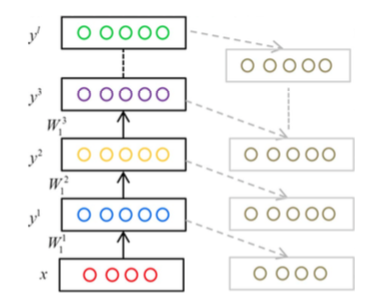
\includegraphics{sae_training.png}}
\caption{Layerwise training of a Stacked Autoencoder}
\label{fig:layerwise-training}
\end{figure}


The basic idea behind layerwise training is shown in Figure~\ref{fig:layerwise-training}. The idea  here is to train each layer as described in Equation~\ref{eqn:sparse}. After a layer is trained, the autoencoder output layer is discarded and the features (the $\mathbf{y}^{(i)}$) are used as the input to the next layer. Hence the training is greedy and layerwise. Finally, the last layer in the network, usually either a linear regression layer (if the output values are continuous) or logistic regression layer (if the output is discrete). The final step is to fine tune the network in a supervised fashion using the back propagation algorithm~\cite{WIDROW2002}.

\section{Data Sets, Performance Metrics and Model Performance}
\label{sec:datasets}

In the initial study we collect data from $\Psi$ sensors (interfaces)\footnote{$\Psi$ is dependent both on network topology and instrumentation.} both in the aggregation and core layers of the data center network on 5 minute intervals for one year, yielding 105,120 samples. These sensors can be thought of as the following RFC 7223~\cite{RFC7223} counters: speed,discontinuity-time,in-octets, in-unicast-pkts, in-broadcast-pkts, in-multicast-pkts,in-discards,in-errors, in-unknown-protos, out-octets, out-unicast-pkts, out-broadcast-pkts, out-multicast-pkts, out-discards,out-errors which are collected on a per-interface basis. 

\subsection{Congestion Computation}
\label{sec:congestion}
For purposes of this study it would be useful to have a sensor that indicated output queue length, such as the RFC 2863~\cite{RFC2863} ifOutQLen counter which in theory could directly measure congestion as a function of output queue length. Given that RFC 7223 counters are not universally implemented, RFC 2863 counters are used where RFC 7223 counters are not available. 

{\color{red} Note: need to compute a robust congestion statistic if I can't get it directly e.g., ifOutQLen ; there is also a question as to L2 vs. L3 queues}


Finally, more complex methods of estimating congestion (e.g., ~\cite{LUI2007}) could be used in future versions.

\subsection{Data Dimensionality}
Recall that the the problem is to measure the sequence $\{X_{i}^{t}\}$ of observed traffic flow data (the 15 parameters described above plus a timestamp) , 
$i = 1, 2, ..., m$ and $t = 1, 2, ..., T$  and predict the traffic flow (and hence potential congestion) at the time $(t + \Delta)$ for some prediction horizon $\Delta$.  
Here $T = (60*24*365)/5 = 105120$. Note that we also want to consider the temporal relationships inherent in traffic flows, so to predict the traffic flow at time interval $t$, 
we also use the traffic flow data at previous time intervals, i.e., $X^{t-1}, X^{t-2}, . . . , X^{t-r}$ for some value of $r$. Thus while the the exact network topology is a 
hyper-parameter in this study, the model described here incorporates both temporal and spatial correlations; the dimension $d$ of the input data is $\Psi * r *(15 + 1)$.

{\color{red} Note: I want to train the top layer (linear regression) on specific links of interest in the network; we use all the data to train the SAE layers (this provides the model with both temporal and spatial correlations (if they exist) inherently}



\subsection{Performance Metrics}
\label{sec:metrics}
In order to evaluate the effectiveness of the proposed model, we use three performance indexes:  Mean Absolute Error (MAE), Mean Relative Error (MRE), and the Root Mean Squared Error  (RMSE). These  are defined as follows: \\
\begin{center}
\begin{tabular}{l}
$\text{MAE} = \frac{1}{n}\sum\limits_{i = 1}^{n} |f_i - \hat{f}_i|$ \\
$\text{MRE} = \frac{1}{n}\sum\limits_{i = 1}^{n} \frac {|f_i - \hat{f}_i|}{f_i}$ \\
$\text{RMSE} = \left[\frac{1}{n}\sum\limits_{i = 1}^{n} \left ({|f_i - \hat{f}_i|}\right)^2\right]^{\frac{1}{2}}$ \\
\label{table:metrics} 
\end{tabular}
\end{center}

where where $f_i$ is the observed traffic flow and $\hat{f}$  is the predicted traffic flow.

%
%\begin{equation}
%\text{MAE} = \frac{1}{n}\sum\limits_{i = 1}^{n} |f_i - \hat{f}_i|
%\label{eqn:mae}
%\end{equation}
%
%
%\begin{equation}
%\text{MRE} = \frac{1}{n}\sum\limits_{i = 1}^{n} \frac {|f_i - \hat{f}_i|}{f_i}
%\label{eqn:mre}
%\end{equation}
%
%\begin{equation}
%\text{RMSE} = \left[\frac{1}{n}\sum\limits_{i = 1}^{n} \left ({|f_i - \hat{f}_i|}\right)^2\right]^{\frac{1}{2}}
%\label{eqn:rmse}
%\end{equation}

\subsection{Results}
\label{sec:results}


\section{Conclusions and Future Work}
 \label{sec:conclusions}

\section{Acknowledgements}

\newpage
% \cite{test}
\bibliographystyle{plain}
\bibliography{/Users/dmm/papers/bib/ml}
% \bibliography{/Users/dmm/papers/bib/rfc}


\end{document}  


% \begin{equation}
% KL(\rho\parallel\hat{\rho}) = \rho \log\frac{\rho}{\hat{\rho_{j}}} + (1 - \rho) \log \frac{1 - \rho}{1 - \hat{\rho_{j}}}
% \label{eqn:KL}
% \end{equation}

% \begin{equation}
% \begin{array}{cc}\text{minimize} \\ {W_{1}, W_{2}}\end{array}
% \sum\limits_{i = 1}^{m}
% (\parallel {W_{2}W_{1}^{T}x^{(i)} - x^{(i)}}\parallel_{2}^{2}
% + \lambda\sum\limits_{j = 1}^{k}\sqrt{\epsilon + H_{j}(W_{1}^{T}x^{(i)})^{2}})
% \label{eqn:google}
% \end{equation}
